% FELIPE BANDEIRA DA SILVA
%
% MANUAL DO SOFTWARE DE SISTEMAS DE ATERRAMENTO
% LAMOTRIZ 2013-2015
% FORTALEZA-CE
% UFC - UNIVERSIDADE FEDERAL DO CEARÁ

\documentclass[a4paper, 10pt]{article}
%\documentclass[paper=a4, fontsize=11pt]{article}

\usepackage[brazil]{babel}
\usepackage[utf8]{inputenc}
\usepackage{listings}
\usepackage{color}
\usepackage{amsthm}
\usepackage{graphicx}
\usepackage{cite}
\usepackage{schemabloc}
\usetikzlibrary{circuits}

\usepackage{float}

\usepackage{hyperref}

\usepackage{multirow}

\usepackage{lipsum}

\setlength{\parindent}{0pt}
\setlength{\parskip}{18pt}

\title{Manual de Uso\\SISTEMAS DE ATERRAMENTO}
\author{LAMOTRIZ}
%\date{}


\begin{document}

\maketitle

Objetivo: Apresentação dos aspectos gerais de funcionamento, 
exemplos e  especificações técnicas.
\footnote{Versão do Manual 1.0}.


\newpage

\tableofcontents

\newpage

\listoffigures

\newpage

%%%%%%%%%%%%%%%%%%%%%%%%%%%%%%%%%%%%%%%%%%%%%%%%%%
%%%%%%%%%%%%%%%%%%%%%%%%%%%%%%%%%%%%%%%%%%%%%%%%%%
%%%%%%%%%%%%%%%%%%%%%%%%%%%%%%%%%%%%%%%%%%%%%%%%%%
%%%%%%%%%%%%%%%%%%%%%%%%%%%%%%%%%%%%%%%%%%%%%%%%%%
%%%%%%%%%%%%%%%%%%%%%%%%%%%%%%%%%%%%%%%%%%%%%%%%%%
\section{Descrição}

O equipamento é capaz de analisar o número de hastes
(eletrodos de aterramento) para a topologia de aterramento
de hastes em linha reta (paralelo), por exemplo, 3 hastes em paralelo. 
Para isto utiliza medições antigas para o processo de treinamento e 
classificação. Este equipamento não é adequado para medição de 
resistência de aterramento, resistividade do terreno ou detectar correntes 
parasitas presentes no solo, para isto, utilize um terrômetro. 

O equipamento é apresentado na Figura \ref{fig_fonte}. Sendo composto pelos 
seguintes itens:


\begin{enumerate}
    \item Gerador/Fonte de impulso de alta tensão.
    \item Computador.
\end{enumerate}


\begin{figure}[!h]
        \caption{\label{fig_fonte}Itens principais do sistema. (1) - Fonte de Impulso, (2) - Computador}
	    \begin{center}
	        \includegraphics[scale=0.1]{../fotos/CAM00189.jpg}
	    \end{center}
\end{figure}

O equipamento opera com nível de tensão elevado, portanto, cuidado no 
manuseio do mesmo e durante o processo de identificação. Que demora em
média de 1 a 5 minutos, dependendo do número de amostras desejadas.

Cuidado com o manuseio do computador levado em campo, especialmente 
no disco rígido. Nele contém os dados das amostras feitas que futuramente
são utilizadas para as melhorias no software de identificação. 
%%%%%%%%%%%%%%%%%%%%%%%%%%%%%%%%%%%%%%%%%%%%%%%%%%
%%%%%%%%%%%%%%%%%%%%%%%%%%%%%%%%%%%%%%%%%%%%%%%%%%
%%%%%%%%%%%%%%%%%%%%%%%%%%%%%%%%%%%%%%%%%%%%%%%%%%


\section{Conexões e Alimentação}

A Figura \ref{fig_painel_frontal} apresenta a vista frontal da Gerador de 
Impulso de Alta Tensão.
Mostrando os seguintes itens, 

\begin{enumerate}
    \item Borne Vermelho, deve-se conectar o cabo que está fixado no 
        ponto de inspeção do sistema de aterramento a ser identificado.
    \item Borne Verde, não utilizado.
    \item Borne Preto, não utilizado
\end{enumerate}

Os demais itens vistos e, não comentados, são para uso exclusivo no desenvolvimento do equipamento. Não devem
ser utilizados para os fins do usuário. 

\textbf{OBS: A chave ON/OFF deve estar sempre na posição ON.} A posição \textit{OFF} deve ser 
evitada, podendo tornar os resultados não confiáveis. Exclusiva para o desenvolvimento
em laboratório.

\begin{figure}[!h]
        \caption{\label{fig_painel_frontal} Vista do painel frontal, identificação dos conectores.}
	    \begin{center}
            \includegraphics[scale=0.1]{../fotos/painel_frontal.jpg}
	    \end{center}
\end{figure}

%%\subsection{Conexão Modo 1}
%%
%%O processo de identificação pode ser feito de dois modos. O primeiro apresentado nesta seção é
%%referente à não utilização do eletrodo de tensão. Exemplificado pela Figura \ref{fig_conexao_modo1}.
%%\textbf{IMPORTANTE:} Este modo requer a correta localização da fase e neutro da linha de alimentação 
%%para a Fonte. Informações mais detalhadas seção: \nameref{sec_alimentacao}.

\subsection{Ligação da Haste Auxiliar e Malha de Terra}

A Figura \ref{fig_conexao_modo1} exemplifica como deve ser feito a ligação das hastes 
ao Gerador de Impulso. 

\begin{figure}[!h]
        \caption{\label{fig_conexao_modo1}Conexão gerador com a malha.}
	    \begin{center}
            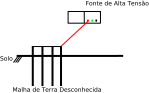
\includegraphics[scale=1.2]{../fotos/conexoes/hastes_modo_1.pdf}
	    \end{center}
\end{figure}


%%\subsection{Conexão Modo 2}
%%
%%Este modo utiliza de uma segunda haste para o processo de identificação de uma malha de 
%%aterramento. Possuindo agora duas, que são nomeadas de: Haste Auxiliar-Central e Haste 
%%Auxiliar-Retorno. Exemplificação Figura \ref{fig_conexao_modo2}.
%%
%%\begin{figure}[!ht]
%%        \caption{\label{fig_conexao_modo2}Conexão Modo 2.}
%%	    \begin{center}
%%            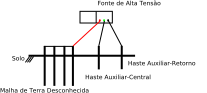
\includegraphics[scale=1.2]{../fotos/conexoes/hastes_modo_2.pdf}
%%	    \end{center}
%%\end{figure}




%%%%%%%%%%%%%%%%%%%%%%%%%%%%%%%%%%%%%%%%%%%%%%%%%%
%%%%%%%%%%%%%%%%%%%%%%%%%%%%%%%%%%%%%%%%%%%%%%%%%%
%%%%%%%%%%%%%%%%%%%%%%%%%%%%%%%%%%%%%%%%%%%%%%%%%%
\newpage
\subsection{Alimentação}
\label{sec_alimentacao}


%Para que a fonte opere corretamente é necessário duas condições. É necessário um 
%ponto de energia que forneça uma tensão de aproximadamente 220 Volts. O segundo 
%ponto e principal, a correta identificação da Fase na instalação.

Para que a Fonte de Impulso opere corretamente, é necessário que a fonte de alimentação 
forneça uma tensão de 220 Volts. Também é necessário a correta 
identificação dos pinos de Fase e Neutro da instalação. \textbf{Omissão desta necessidade 
pode provocar de erros na leitura a danos aos componentes internos da Fonte de Impulso.}

\begin{figure}[!h]
        \caption{\label{fig_vista_traseira_fonte} Vista traseira da fonte.}
	    \begin{center}
            \includegraphics[scale=0.08]{../fotos/fonte_alimentacao.jpg}
	    \end{center}
\end{figure}

A Figura \ref{fig_vista_traseira_fonte} mostra à chave principal de ligar ou 
desligar o gerador de impulso, ao seu lado o conector fêmea para entrada da alimentação de 220V.
Bem como a localização do Neutro e Fase do equipamento. 


A exemplificação do esquema de ligação da alimentação é vista 
na Figura \ref{fig_esquema_ligacao_alimentacao}. Contendo duas vistas, vista frontal da fonte e vista
traseira. Bem como, a localização do neutro e fase da instalação e fonte de impulso.

\begin{figure}[!h]
        \caption{\label{fig_esquema_ligacao_alimentacao} Esquema de ligação da alimentação.}
	    \begin{center}
            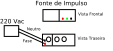
\includegraphics[scale=1.2]{../fotos/conexoes/alimentacao.pdf}
	    \end{center}
\end{figure}

% 29 jan 15
%\textbf{*****MUDARISSO***** A fase é identificada no conector como sendo, o pino inferior
%visto de baixo para cima. ***APRESENTAR NA FIGURA***}



%%%%%%%%%%%%%%%%%%%%%%%%%%%%%%%%%%%%%%%%%%%%%%%%%%
%%%%%%%%%%%%%%%%%%%%%%%%%%%%%%%%%%%%%%%%%%%%%%%%%%
%%%%%%%%%%%%%%%%%%%%%%%%%%%%%%%%%%%%%%%%%%%%%%%%%%
\section{Instalação do Software}

Para que o software de aterramento funcione corretamente, 
são necessários os seguintes softwares na máquina a ser utilizada nos ensaios:

\begin{enumerate}
    \item Windows8
    \item Python 2.7
    \item PyQT 4
    \item PyVisa 1.4
    \item Matplotlib
    \item Numpy
    \item Scipy
\end{enumerate}

É disponibilizado para tanto, um instalador para todos estes software. Presente 
na mídia física junto ao equipamento. 
É possível baixar pelo link: 
% copy
\url{https://copy.com/2KwTthmf9Lqy6NU}
% dropbox
%\url{https://www.dropbox.com/s/o8wal1l2ejuq56h/setup-sistemas-aterramento.24feb15.v1.exe?dl=0}

\textbf{Observação:} É necessário uma conexão com a internet para a correta 
instalação das dependências, em especial do  \textit{pyvisa\footnote{Controle de Instrumentos com Python. Mais informações em http://pyvisa.readthedocs.org/en/master}}.


\subsection{Passo a Passo da Instalação}

O instalador para todos os softwares necessários é disponibilizado em um único
binário. Bastando apenas para o usuário guiar à instalação. A Figura \ref{fig_iniciando_instalacao} apresenta visão inicial para os passos seguintes.

\begin{figure}[!h]
        \caption{\label{fig_iniciando_instalacao}Iniciando a instalação.}
	    \begin{center}
            \includegraphics[scale=0.7]{../fotos/instalacao/parte1_executando.pdf}
	    \end{center}
\end{figure}

Uma vez executado o instalador, na segunda tela, é possível selecionar o componentes 
que serão instalados, caso já não foram. São os principais \textit{Anaconda}, \textit{PyQT} e o software
alvo do projeto de pesquisa. O \textit{Anaconda} contém as principais ferramentas para se
trabalhar com o \textit{Python}, processamento de imagens e cálculo numérico. O \textit{PyQT} é 
o \textit{GUI}\footnote{Interface Gráfica} utilizado para a construção da interface entre o usuário e por fim 
o software para analisar e identificar uma topologia de aterramento. Passo este apresentado 
na Figura \ref{fig_selecionando_componentes_externos}. 

É recomendado a instalação de todos os componentes presentes no instalador, como é 
visto na Figura \ref{fig_selecionando_componentes_externos}. 

\begin{figure}[!h]
        \caption{\label{fig_selecionando_componentes_externos}Selecionando os componentes necessários.}
	    \begin{center}
            \includegraphics[scale=0.7]{../fotos/instalacao/parte2_selecionando_componentes.pdf}
	    \end{center}
\end{figure}

Uma vez confirmado os componentes necessário, o processo, propriamente dito, de instalação 
é iniciado. Em um determinado momento da instalação aparecerão na tela, outros dois instaladores. 
São eles do \textit{Anaconda} e \textit{PyQt}, este devem ser guiados também pelo usuário.

\begin{figure}[!h]
    \caption{\label{fig_pyqt_antigo}Confirmando a desinstalação do \textit{PyQT} básico para a instalação do completo.}
	    \begin{center}
            \includegraphics[scale=0.6]{../fotos/instalacao/parte6_pyqt.pdf}
	    \end{center}
\end{figure}


No momento da instalação do \textit{PyQT} aparece uma mensagem, Figura \ref{fig_pyqt_antigo},  informando que 
já existe uma instalação na pasta do \textit{Anaconda}, no entanto esta é a instalação básica do \textit{PyQT}. 
Confirme a desinstalação do componente e continue a instalação completa do \textit{PyQT}.


%\begin{figure}[!ht]
%        \caption{\label{fig_processo_inicial_instalacao}Processo inicial da instalação.}
%	    \begin{center}
%            \includegraphics[scale=0.6]{../fotos/instalacao/parte3_descompactando.pdf}
%	    \end{center}
%\end{figure}

No final é criado um atalho chamado ``aterramento'' na área de trabalho.


%%%%%%%%%%%%%%%%%%%%%%%%%%%%%%%%%%%%%%%%%%%%%%%%%%
%%%%%%%%%%%%%%%%%%%%%%%%%%%%%%%%%%%%%%%%%%%%%%%%%%
%%%%%%%%%%%%%%%%%%%%%%%%%%%%%%%%%%%%%%%%%%%%%%%%%%
\section{Apresentação do Software}

A Figura \ref{fig_tela_inicial} apresenta a tela inicial em modo tela cheia do \textit{software} Aterramento 1.0. 
Com este \textit{software} é possível interagir totalmente com a fonte de impulso, sistema de aquisição de 
tensão e corrente bem como analisar as amostrar e obter os resultados e plotagem de 
gráficos armazenados na memória.

\begin{figure}[!h]
    \caption{\label{fig_tela_inicial}Tela Inicial do Aterramento 1.0.}
	    \begin{center}
            \includegraphics[scale=0.3]{../fotos/execucao/tela_inicial.png}
	    \end{center}
\end{figure}

A interface é divida em partes. As principais são:

\begin{itemize}
    \item Entradas.
    \item Ações.
    \item Resultados.
\end{itemize}

Outras partes são referente a como deve ser feito a ligação dos fios e apresentação dos
apoiadores e executores do projeto.

\subsection{Entrada}

Antes de iniciar o processo de análise, são necessárias algumas configurações
iniciais. O primeiro passo é definir onde serão salvos os dados das amostras, 
isto é feito selecionando uma ``área de trabalho''. 
Clicando no ``botão'' ao lado da referência ``área de trabalho''.
Ao fazer isto abre-se uma janela para selecionar uma pasta que 
servirá para tal propósito.


O número de amostra garante a confiabilidade na análise, em
compensação, aumenta o tempo necessário para aquisição dos dados de tensão e corrente. O valor 30, 
é recomendado e foi definido como padrão. 
O tempo estimando para a coleta de uma única amostra, é de aproximadamente 5,6 segundos. 
Portanto para uma coleta de 30 amostra é necessário aproximadamente 2,8 minutos. Podendo variar de 
acordo com as especificações do computador utilizado.

O armazenamento das amostra é feito utilizando a data atual, o nome do terreno e o arranjo esperado para 
o mesmo. Valores estes que podem ser definidos ainda na ``Entrada'', podendo serem alterados a qualquer
momento. 

Em campo é bastante útil a visualização da onda adquirida pelo sistema de aquisição, portanto para 
que seja possível visualizá-la após o processo de análise. Marca-se a opção ``Plotar o transiente 
após análise''.

\subsection{Ações}

A segunda parte ``Ações'', é responsável por dar início ao processo de identificação de uma topologia
de aterramento. Esse processo consiste em acionar a fonte de impulso ``n'' vezes e capturar 
os sinais de tensão e corrente. Após isto estes valores são salvos na memória, para então serem 
classificados pelo software.

\textbf{IMPORTANTE:} Este equipamento opera com níveis de tensão elevados, portanto ao clicar em 
``Iniciar'' garanta que ninguém esteja perto das hastes ou da malha alvo da identificação. Não toque
nos cabos e conectores da fonte.

Uma vez iniciado o processo uma barra mostrará o progresso. Caso seja necessário, é possível cancelar, 
clicando no botão ``Cancelar'', sendo assim é pedido um tempo menor que 5 segundos para o cancelamento
por completo.

\subsection{Resultados}

%Ao fim do processo de análise são apresentados os resultados para o usuário. São dois resultados, o 
%primeiro apresenta o resultado aproximado encontrado pelo programa. O segundo apresenta o resultado 
%exato, sendo este a resposta final para o usuário.

Ao fim do processo de coleta de amostra e análise, é apresentado para o usuário o resultado. 
Na campo ``Número exato'' é possível visualizar a topologia identificada. Com uma taxa de 
acerto de aproximadamente $92 \%$.

Apresenta-se também o tempo real que foi necessário para todo o ensaio. Tempo este que pode variar
das configurações do computador  ao número de amostras escolhidas.

\subsection{Terminal}

Uma ferramento bastante útil, é o terminal que carregado na inicialização do software.

\begin{figure}[!h]
    \caption{\label{fig_terminal}Terminal útil para debug.}
	    \begin{center}
            \includegraphics[scale=0.3]{../fotos/execucao/terminal.pdf}
	    \end{center}
\end{figure}

Não sendo fundamental para o usuário final. No entanto, apresenta mensagens informando erros ou avisos,
que foram colocadas no decorrer do programa, tornando o terminal uma ferramenta bastante útil, 
quando algo não estiver funcionando como deveria.

%%%%%%%%%%%%%%%%%%%%%%%%%%%%%%%%%%%%%%%%%%%%%%%%%%
%%%%%%%%%%%%%%%%%%%%%%%%%%%%%%%%%%%%%%%%%%%%%%%%%%
%%%%%%%%%%%%%%%%%%%%%%%%%%%%%%%%%%%%%%%%%%%%%%%%%%
\section{Exemplo, Identificando um Malha de Terra}

O Exemplo aqui abortado é referente a identificação de uma topologia de aterramento
desconhecida até então, ficando apenas no entendimento do processo necessário de 
ligação ao acionamento do software.

Todo o processo de identificação esta sujeito a erros, portanto deve ser feito a 
interpretação do resultado quando apresentado.

\subsection{Ligando a Fonte}

Antes de ligar a fonte de alta tensão a rede elétrica, certifique-se,

\begin{enumerate}
    \item Identifique corretamente a Fase e Neutro na linha de alimentação da fonte.
    \item O cabo USB deve esta devidamente conectado a uma porta livre do computador.
    \item Software responsável pela identificação esta devidamente inicializado e aguardando
        os comandos do usuário.
    \item A ligação com a malha de terra. 
\end{enumerate}

\textit{A omissão do passo 1 mostrado acima, pode ocasionar de erros na leitura a 
danos aos componentes internos da fonte de alta tensão.}

Na Figura \ref{fig_ligacao_hastes} é possível visualizar todas as ligações necessárias.

\begin{figure}[H]
        \caption{\label{fig_ligacao_hastes}Exemplo de Ligação}
	    \begin{center}
            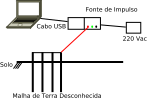
\includegraphics[scale=1.2]{../fotos/conexoes/hastes.pdf}
	    \end{center}
\end{figure}

\subsection{Preparando o Software}

Para que o \textit{Software} funcione corretamente é necessário selecionar uma 
área de trabalho e se necessário, quantidade de amostras a serem feitas. 
Para melhorar na identificação posterior de ensaios feitos é importante nomear 
o terreno alvo do ensaio, bem como um rótulo para à malha de terra a ser 
estudada. Como mostra a Figura \ref{fig_entrando_os_dados} .

\begin{figure}[H]
        \caption{\label{fig_entrando_os_dados}Dados de Entrada.}
	    \begin{center}
            \includegraphics[scale=0.4]{../fotos/execucao/selecionando_area_trabalho_2.png}
	    \end{center}
\end{figure}

Se caso necessário, em uma situação que o resultado pode não ser confiável, 
é possível visualizar o gráfico da tensão e corrente das amostras. Para isto 
é necessário confirmar a caixa ``Plotar o transiente após análise''.

\subsection{Identificação e Resultados}

Inicie o ensaio clicando em ``INICIAR'', visto na Figura \ref{fig_iniciando_ensaio}.

\begin{figure}[H]
        \caption{\label{fig_iniciando_ensaio}Iniciando o Ensaio.}
	    \begin{center}
            \includegraphics[scale=0.4]{../fotos/execucao/iniciando_amostragem.png}
	    \end{center}
\end{figure}

Depois de aproximadamente 3 minutos um resultado deve ser apresentando, um exemplo
pode ser visto na Figura \ref{fig_ex_resultado}.

\begin{figure}[H]
        \caption{\label{fig_ex_resultado}Exemplo de Resultado.}
	    \begin{center}
            \includegraphics[scale=0.4]{../fotos/execucao/resultados.png}
	    \end{center}
\end{figure}


É possível plotar o gráfico, em outro momento, navegando até a opção:

Análise $\rightarrow$ Plotar Gráfico $\rightarrow$ Plot V I transiente. 

Contida na barra de tarefas, localizada na parte superior da janela principal.

\begin{figure}[H]
        \caption{\label{fig_plt_transiente}Plot do Transiente.}
	    \begin{center}
            \includegraphics[scale=0.4]{../fotos/execucao/plot_transiente.png}
	    \end{center}
\end{figure}




%%%%%%%%%%%%%%%%%%%%%%%%%%%%%%%%%%%%%%%%%%%%%%%%%%
%%%%%%%%%%%%%%%%%%%%%%%%%%%%%%%%%%%%%%%%%%%%%%%%%%
%%%%%%%%%%%%%%%%%%%%%%%%%%%%%%%%%%%%%%%%%%%%%%%%%%
%\section{Princípio de Funcionamento}
%
%Um dos principais objetivos na construção de uma malha de terra é a 
%proteção da vida humana. Serve também para que os equipamentos de 
%proteção, por exemplo, de uma subestação funcionem corretamente como
%o pará-raio. Portanto a malha de terra é um item fundamental e 
%demanda cuidados do projeto, construção a utilização.
%
%Entretanto devido a falhas na execução do projeto, é possível que a quantidade
%de hastes não sejam colocadas em sua totalidade. Trazendo riscos para o 
%funcionamento do sistema, e levando a possíveis prejuízos fiscais para a 
%empresa contratante. Em outros casos é possível que exista uma falha na 
%conexão elétrica em algum ponto da malha.
%
%Este equipamento inovador é portanto uma solução a identificação de uma topologia
%de aterramento já construída é que necessita de uma verificação se foi corretamente
%executada ou se não existem falhas elétricas.
%
%Para o estudo de uma malha de terra quando submetida a uma descarga atmosférica 
%é possível encontrar na literatura, modelos de circuitos elétricos, modelos 
%eletromagnéticos, linhas de transmissão entre outros. Em todos é nota-se 
%que os parâmetros mais majoritários são: solo e características das hastes. 
%Parâmetros estes que determinam, resposta da malha de terra. Então o objetivo
%deste equipamento é diferenciar as possíveis topologias de malha de terra. 
%
%Utilizando uma Máquina de Aprendizado para o reconhecimento de padrões, 
%partindo de uma situação já conhecidas. O sistema é divido em quatro partes, 
%
%\begin{enumerate}
%    \item Excitação.
%    \item Aquisição.
%    \item Extração das Características.
%    \item Reconhecimento dos Padrões.
%\end{enumerate}
%
%%%%%%%%%%%%%%%%%%%%%%%%%%%%%%%%%%%%%%%%
%\subsection{Excitação}
%
%Para que o reconhecimento seja feito é necessário aplicar um determinado pulso
%de tensão na topologia de aterramento, até então desconhecido. 
%Sendo esta função de responsabilidade do Gerador de Impulso de Tensão. 
%Sendo apresentado na Figura \ref{fig_principio_funcionamento} e 
%anteriormente na Figura \ref{fig_fonte}.
%
%\begin{figure}[!h]
%        \caption{\label{fig_principio_funcionamento}Princípio de Funcionamento do Sistema.}
%	    \begin{center}
%            \includegraphics[scale=0.3]{../fotos/principio/principio_de_funcionamento_corte.pdf}
%	    \end{center}
%\end{figure}
%
%Sabe-se, quando a malha é submetida a frequência de 60 Hz os efeitos indutivos e 
%capacitivos da mesma são desprezíveis. Entrando ao aplicar um pulso de 
%alta tensão com uma constante de tempo pequena, constante que irá 
%depender diretamente das malha de terra. É possível extrair informações
%úteis. 
%
%A fonte de impulso é portanto o elemento que irá extrair a impedância
%característica de cada malha, com a leitura de corrente e tensão. 
%Para isto é aplicado um pulso de tensão na malha, de aproximadamente
%1000 Volts. 
%
%A resposta é vista na figura \ref{fig_sinal}. 
%
%\begin{figure}[!h]
%    \caption{\label{fig_sinal} Sinal típico da resposta.}
%	    \begin{center}
%            \includegraphics[scale=0.5]{../fotos/sinal/sinal-eps-converted-to.pdf}
%	    \end{center}
%\end{figure}
%
%%%%%%%%%%%%%%%%%%%%%%%%%%%%%%%%%%%%%%%%
%\subsection{Aquisição}
%
%O processo de aquisição começa quando o pulso é disparado na topologia de aterramento.
%Mensurando e armazenando toda a leitura de tensão e corrente simultaneamente, a um velocidade
%de 2MSa/s com resolução de 14 bits. 
%Tal velocidade garante a maior número de pontos adquiridos em um curto espaço de tempo, 
%aumentando assim a eficácia do resultado.
%
%Ampliando o sinal armazenado é possível notar, em uma configuração exemplo, com 30
%amostras. A resposta para aquela topologia, sendo o início desta resposta à mais 
%importante. Isto acontece em aproximadamente 125 us em média. Como pode ser visto
%na Figura \ref{fig_sinal_detalhe}.
%
%\begin{figure}[!h]
%    \caption{\label{fig_sinal_detalhe} Sinal ampliado no pico de tensão da resposta.}
%	    \begin{center}
%            \includegraphics[scale=0.5]{../fotos/sinal/sinal_detalhes-eps-converted-to.pdf}
%	    \end{center}
%\end{figure}
%
%O processo de aquisição consiste em adquirir tensão e corrente, tensão 
%que é aplicada na malha de aterramento e corrente que flui pela mesma. 
%Este processo é visto na Figura \ref{fig_ideia_aquisicao}. Onde utiliza-se
%o aterramento do lado de baixa tensão do transformador, como ponto de retorno
%de corrente e extremidade para sensor de tensão. Por isto é essencial a 
%correta ligação do fase e neutro da fonte de impulso visto do capítulo \ref{sec_alimentacao}
%e Figura \ref{fig_esquema_ligacao_alimentacao}.
%
%\textbf{OBS:} Portanto fica claro, é necessário que o lado de baixa tensão
%do transformador deva ser \textbf{estrela aterrado}. Se está condição não for 
%satisfeita o processo de identificação de uma topologia de aterramento não 
%funcionará.
%
%\begin{figure}[!h]
%    \caption{\label{fig_ideia_aquisicao} Idealização da aquisição.}
%	    \begin{center}
%            \includegraphics[scale=0.4]{../fotos/sinal/trafo.png}
%	    \end{center}
%\end{figure}
%
%%%%%%%%%%%%%%%%%%%%%%%%%%%%%%%%%%%%%%%%%
%\subsection{Extração das Características}
%
%Busca-se das formas de onda de tensão e corrente características típicas para 
%cada topologia, aplicando FFT(\textit{Fast Fourier Transform}) a impedância 
%no domínio do tempo($t$) resultante $z_n=v_n(t)/i_n(t)$ para cada amostra ($n$).
%Obtendo assim os harmônicos do sinal. Também é levado em consideração
%o decaimento total da onda.
%
%%Com isto é possível encontrar padrões para cada topologia de aterramento, independente
%%do solo e condições climáticas.
%
%Com esta abordagem é possível encontrar padrões para cada topologia de aterramento, 
%independente do solo e condições climáticas.
%
%%%%%%%%%%%%%%%%%%%%%%%%%%%%%%%%%%%%%%%%%
%\subsection{Reconhecimento dos Padrões}
%
%Durante o processo de desenvolvimento do projeto sistemas de 
%aterramentos, três modelos foram utilizados para a classificação.
%São eles, AdaBoost (impulso ou estimulo adaptativo), Support 
%Vector Machine (máquina de vetor de suporte) e Random Forest
%(árvores randomizadas). 
%
%Para encontrar a taxa de acerto dos três modelos, foram utilizado
%26 ensaios. Em um rodizio de 26 rodadas, onde cada rodada contem 
%25 ensaios usados para o treinamento e 1 para
%validação. Exemplificado 
%na Figura \ref{fig_treinamento}.
%
%\begin{figure}[!h]
%    \caption{\label{fig_treinamento}Processo de treinamento para as amostras.}
%	    \begin{center}
%            \includegraphics[scale=0.5]{../fotos/principio/rodizio.png}
%	    \end{center}
%\end{figure}
%
%Com a finalização do processo de treinamento, os três algorítimos 
%apresentaram diferentes taxas de acerto para as topologias estudadas.
%Como pode ser visto na tabela \ref{tab:modelo}, para 
%os algoritmos AR(Árvores Randomizadas),  MSV(Máquina de Vetor de Suporte) e Adaboost.
%
%A tabela \ref{tab:modelo} apresenta as taxas de acerto, linha diagonal principal, 
%e as taxas de erros em comparação com o real. Para os três algoritmos escolhidos 
%é possível visualizar que, a taxa de acerto de AR é idêntica para MSV.
%
%
%% Please add the following required packages to your document preamble:
%% \usepackage{multirow}
%% \usepackage[table,xcdraw]{xcolor}
%% If you use beamer only pass "xcolor=table" option, i.e. \documentclass[xcolor=table]{beamer}
%\begin{table}[!t]
%    \centering
%\caption{Taxa de acerto para os modelos AR, Adaboost e MSV}
%\begin{tabular}{|c|l|l|l|l|l|}
%\hline
%\textbf{AR} & \multicolumn{5}{c|}{Saída do Modelo Proposto} \\ \hline
% &  & 1 haste & 2 hastes & 3 hastes & 4 hastes \\ \cline{2-6} 
% & 1 haste & 100 \% & 0 \% & 0 \% & 0 \% \\ \cline{2-6} 
% & 2 hastes & 2,9 \% & 97,1 \% & 0 \% & 0 \% \\ \cline{2-6} 
% & 3 hastes & 0 \% & 2,9 \% & 97,1 \% & 0 \% \\ \cline{2-6} 
%\multirow{-5}{*}{\begin{tabular}[c]{@{}c@{}}Topologia\\ Real\end{tabular}} & 4 hastes & 0 \% & 2,9 \% & 0 \% & 97,1 \% \\ \hline
%\multicolumn{1}{|l|}{\begin{tabular}[c]{@{}l@{}}Taxa de \\ Acerto\end{tabular}} & \multicolumn{5}{c|}{{\color[HTML]{9A0000} \textbf{97,9 \%}}} \\ \hline
%\textbf{Adaboost} &  & 1 haste & 2 hastes & 3 hastes & 4 hastes \\ \hline
% & 1 haste & 97,1 \% & 2,9 \% & 0 \% & 0 \% \\ \cline{2-6} 
% & 2 hastes & 2,9 \% & 97,1 \% & 0 \% & 0 \% \\ \cline{2-6} 
% & 3 hastes & 0 \% & 2,9 \% & 97.1 \% & 0 \% \\ \cline{2-6} 
%\multirow{-4}{*}{\begin{tabular}[c]{@{}c@{}}Topologia\\ Real\end{tabular}} & 4 hastes & 0 \% & 2,9 \% & 2,9 \% & 94,3 \% \\ \hline
%\multicolumn{1}{|l|}{\begin{tabular}[c]{@{}l@{}}Taxa de \\ Acerto\end{tabular}} & \multicolumn{5}{c|}{{\color[HTML]{9A0000} \textbf{96,4 \%}}} \\ \hline
%\textbf{MSV} &  & 1 haste & 2 hastes & 3 hastes & 4 hastes \\ \hline
% & 1 haste & 97,1 \% & 2,0 \% & 0 \% & 0 \% \\ \cline{2-6} 
% & 2 hastes & 0 \% & 97,1 \% & 2,9 \% & 0 \% \\ \cline{2-6} 
% & 3 hastes & 0 \% & 0 \% & 97,1 \% & 2,9 \% \\ \cline{2-6} 
%\multirow{-4}{*}{\begin{tabular}[c]{@{}c@{}}Topologia \\ Real\end{tabular}} & 4 hastes & 0 \% & 0 \% & 0 \% & 100 \% \\ \hline
%\multicolumn{1}{|l|}{\begin{tabular}[c]{@{}l@{}}Taxa de \\ Acerto\end{tabular}} & \multicolumn{5}{c|}{{\color[HTML]{9A0000} \textbf{97,9 \%}}} \\ \hline
%\end{tabular}
%
%\label{tab:modelo}
%\end{table}
%
%%\lipsum[1-2]
%%%%%%%%%%%%%%%%%%%%%%%%%%%%%%%%%%%%%%%%%%%%%%%%%%%
%%%%%%%%%%%%%%%%%%%%%%%%%%%%%%%%%%%%%%%%%%%%%%%%%%%
%%%%%%%%%%%%%%%%%%%%%%%%%%%%%%%%%%%%%%%%%%%%%%%%%%%
%\newpage
\section{Especificações Técnicas}

\begin{table}[h]
    \centering
    \caption{Especificações Técnicas}
\begin{tabular}{|l|l|}
\hline
Aplicação & \begin{tabular}[c]{@{}l@{}}Analisar e identificar uma topologia desconhecida\\ de aterramento. Fornecendo a disposição/topologia\\ das hastes em um aterramento até então desconhecido\end{tabular} \\ \hline
Método de  Identificação & \begin{tabular}[c]{@{}l@{}}É injetado no solo uma corrente elétrica, mede-se o\\ sinal de tensão e corrente resultante. Com isto analisa-se\\ por meio de algoritimos inteligentes qual topologia.\end{tabular} \\ \hline
Precisão & Aproximadamente 98\% \\ \hline
Alimentação & Rede de 220 V / 60 Hz \\ \hline
Porta de Comunicação & USB 2.0 \\ \hline
Peso & 18 Kg, sem a presença do computador \\ \hline
Temperatura de Operação & 20ºC a 50ºC \\ \hline
\end{tabular}

\label{tab:especificacoes}
\end{table}


\end{document}
